\documentclass[format=acmsmall, review=false, screen=true]{acmart}		% ICFP
%\documentclass[format=sigplan, review=true]{acmart}		% HASKELL SYMPOSIUM 
%\documentclass[format=sigconf, review=true]{acmart}		% IFL

%\usepackage{float}
%\usepackage{graphicx}
%\usepackage{subcaption}
%\usepackage{ifthen}
\usepackage{minted}
%\usepackage{verbatim}

% Metadata Information
%% use defaults for review submission.
%\acmConference[HS18]{Haskell Symposium}{2018}{09}
%\acmYear{2018}
%\copyrightyear{2018}
\acmConference[IFL'18]{International Symposium on Implementation and Application of Functional Languages}{August 2019}{Lowell, MA, USA}
\acmYear{2019}
\copyrightyear{2019}
%\acmDOI{} % \acmDOI{10.1145/nnnnnnn.nnnnnnn}

% Copyright
%% use 'none' for review submission.
\setcopyright{none}
%\setcopyright{acmcopyright}	% = copyright transfer to ACM
%\setcopyright{acmlicensed} 		% = retaining copyright but granting ACM exclusive publication rights
%\setcopyright{rightsretained}  % = open access on payment of a fee
%\setcopyright{usgov}
%\setcopyright{usgovmixed}
%\setcopyright{cagov}
%\setcopyright{cagovmixed}

% TODO : get the data
% DOI
% \acmDOI{0000001.0000001}

% TODO: fill in
% Paper history
\received{May 2018}
%\received[revised]{March 2018}
%\received[accepted]{March 2018}

% Document starts
\begin{document}

\newminted[HaskellCode]{haskell}{fontsize=\small}

% Title portion. Note the short title for running heads
\title[The Agent's new Cloths]{The Agent's new Cloths}
\subtitle{Towards functional programming in Agent-Based Simulation}

\author{Jonathan Thaler}
%\orcid{TODO}
\email{jonathan.thaler@nottingham.ac.uk}
\author{Thorsten Altenkirch}
\email{thorsten.altenkirch@nottingham.ac.uk}
\affiliation{%
  \institution{University of Nottingham}
  \streetaddress{7301 Wollaton Rd}
  \city{Nottingham}
  \postcode{NG8 1BB}
  \country{United Kingdom}}

\begin{abstract}
TODO: implement synchronous agent interaction

TODO: parallelism for free because all isolated e.g. running multiple replications or parameter-variations

TODO: it is paramount not to write against the established approach but for the functional approach. not to try to come up with arguments AGAINST the object-oriented approach but IN FAVOUR for the functional approach. In the end: don't tell the people that what they do sucks and that i am the saviour with my new method but: that i have a new method which might be of interest as it has a few nice advantages.

So far, the pure functional paradigm hasn't got much attention in Agent-Based Simulation (ABS) where the dominant programming paradigm is object-orientation, with Java, Python and C++ being its most prominent representatives. We claim that functional programming using Haskell is very well suited to implement complex, real-world agent-based models and brings with it a number of benefits. In this paper we will introduce the reader to the functional programming paradigm and explain how it can be applied to implementing ABS. Further we discuss benefits and advantages. As use-case we implemented the seminal Sugarscape model in Haskell.
\end{abstract}

%
% The code below should be generated by the tool at
% http://dl.acm.org/ccs.cfm
% Please copy and paste the code instead of the example below.
%
% TODO needs to be generated
%\begin{CCSXML}
%<ccs2012>
% <concept>
%  <concept_id>10010520.10010553.10010562</concept_id>
%  <concept_desc>Computer systems organization~Embedded systems</concept_desc>
%  <concept_significance>500</concept_significance>
% </concept>
% <concept>
%  <concept_id>10010520.10010575.10010755</concept_id>
%  <concept_desc>Computer systems organization~Redundancy</concept_desc>
%  <concept_significance>300</concept_significance>
% </concept>
% <concept>
%  <concept_id>10010520.10010553.10010554</concept_id>
%  <concept_desc>Computer systems organization~Robotics</concept_desc>
%  <concept_significance>100</concept_significance>
% </concept>
% <concept>
%  <concept_id>10003033.10003083.10003095</concept_id>
%  <concept_desc>Networks~Network reliability</concept_desc>
%  <concept_significance>100</concept_significance>
% </concept>
%</ccs2012>
%\end{CCSXML}
%
%\ccsdesc[500]{Computer systems organization~Embedded systems}
%\ccsdesc[300]{Computer systems organization~Redundancy}
%\ccsdesc{Computer systems organization~Robotics}
%\ccsdesc[100]{Networks~Network reliability}

%
% End generated code
%

\keywords{Agent-Based Simulation, Functional Programming, Haskell}

\maketitle

\section{Introduction}
There exists a large number of simulation packages which allow the convenient creation of System Dynamics simulations by straight-forward visual diagram creation. One simply creates stocks and flows, connects them, specifies the flow-rates and initial parameters and then runs the model. An example for such a visual diagram creation in the simulation package AnyLogic can be seen in Figure \ref{fig:sir_stockflow_diagram}.

\begin{figure}
	\centering
	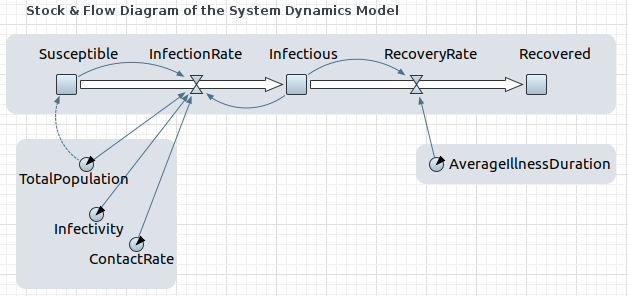
\includegraphics[width=.5\textwidth, angle=0]{./fig/SIR_SD_STOCKFLOW_DIAGRAMM.png}
	\caption{Visual System Dynamics Diagram of the SIR model in AnyLogic Personal Learning Edition 8.3.1.}
	\label{fig:sir_stockflow_diagram}
\end{figure}

Still, implementing System Dynamics directly in code is not as straight forward and involves numerical integration which can be quite tricky to get right. Thus, the aim of this paper is to look into how System Dynamics models can be implemented in code correctly without the use of a simulation package. We use the well known SIR model \cite{kermack_contribution_1927} from epidemiology to demonstrate our approach.

Our language of choice is Haskell because it emphasises a declarative programming style in which one describes \textit{what} instead of \textit{how} to compute. Further it allows to rule out interference with non-deterministic influences or side-effects already at compile-time. This is of fundamental importance for System Dynamics because it behaves completely deterministic and involves no stochastics or non-determinism whatsoever. Also, we make use of Functional Reactive Programming which allows to express continuous-time systems in a functional way. 

We show that by this approach we can arrive at correct-by-construction implementations of System Dynamic models. This means that the correctness of the code is obvious because we have closed the gap between the model specification and its implementation. Thus, the contribution of the paper is the demonstration of how to implement correct-by-construction System Dynamics simulations using Haskell and Functional Reactive Programming.

\section{Bugs and Errors in Agent-Based Simulation}
TODO: general introduction %https://en.wikipedia.org/wiki/Software_bug

The problem of correctness in agent-based simulations became more apparent in the work of Ionescu et al \cite{ionescu_dependently-typed_2012} which tried to replicate the work of Gintis \cite{gintis_emergence_2006}. In his work Gintis claimed to have found a mechanism in bilateral decentralized exchange which resulted in walrasian general equilibrium without the neo-classical approach of a tatonement process through a central auctioneer. This was a major break-through for economics as the theory of walrasian general equilibrium is non-constructive as it only postulates the properties of the equilibrium \cite{colell_microeconomic_1995} but does not explain the process and dynamics through which this equilibrium can be reached or constructed - Gintis seemed to have found just this process. Ionescu et al. \cite{ionescu_dependently-typed_2012} failed and were only able to solve the problem by directly contacting Gintis which provided the code - the definitive formal reference. It was found that there was a bug in the code which led to the "revolutionary" results which were seriously damaged through this error. They also reported ambiguity between the informal model description in Gintis paper and the actual implementation. TODO: it is still not clear what this bug was, find out! look at the master thesis 

This is supported by a talk \cite{sweeney_next_2006}, in which Tim Sweeney, CEO of Epic Games, discusses the use of main-stream imperative object-oriented programming languages (C++) in the context of Game Programming. Although the fields of games and ABS seem to be very different, in the end they have also very important similarities: both are simulations which perform numerical computations and update objects in a loop either concurrently or sequential \cite{gregory_game_2018}. Sweeney reports that reliability suffers from dynamic failure in such languages e.g. random memory overwrites, memory leaks, accessing arrays out-of-bounds, dereferencing null pointers, integer overflow, accessing uninitialized variables. He reports that 50\% of all bugs in the Game Engine Middleware Unreal can be traced back to such problems and presents dependent types as a potential rescue to those problems.

TODO: list common bugs in object-oriented / imperative programming
TODO: java solved many problems 
TODO: still object-oriented / imperative ultimately struggle when it comes to concurrency / parallelism due to their mutable nature.

TODO: \cite{vipindeep_list_2005}

TODO: software errors can be costly %https://raygun.com/blog/costly-software-errors-history/
TODO: bugs per loc %https://www.mayerdan.com/ruby/2012/11/11/bugs-per-line-of-code-ratio

\section{Functional Programming}
The roots of functional programming lie in the Lambda Calculus which was first described by Alonzo Church \citep{church_unsolvable_1936}. This is a fundamentally different approach to computation than imperative and object-oriented programming which roots lie in the Turing Machine \citep{turing_computable_1937}. Rather than describing \textit{how} something is computed as in the more operational approach of the Turing Machine, due to the more declarative nature of the Lambda Calculus, code in functional programming describes \textit{what} is computed.

In our research we are using the functional programming language Haskell. The paper of \citep{hudak_history_2007} gives a comprehensive overview over the history of the language, how it developed and its features and is very interesting to read and get accustomed to the background of the language. The main points why we decided to go for Haskell are:

\begin{itemize}
	\item Rich Feature-Set - it has all fundamental concepts of the pure functional programming paradigm of which we explain the most important below.
	\item Real-World applications - the strength of Haskell has been proven through a vast amount of highly diverse real-world applications \cite{hudak_history_2007}, is applicable to a number of real-world problems \cite{osullivan_real_2008} and has a large number of libraries available \footnote{\url{https://wiki.haskell.org/Applications_and_libraries}}.
	\item Modern - Haskell is constantly evolving through its community and adapting to keep up with the fast changing field of computer science. Further, the community is the main source of high-quality libraries.
\end{itemize}

As a short example we give an implementation of the factorial function in Haskell:
\begin{HaskellCode}
factorial :: Integer -> Integer
factorial 0 = 1
factorial n = n * factorial (n-1)
\end{HaskellCode}

When looking at this function we can already see the central concepts of functional programming: 
\begin{enumerate}
	\item Declarative - we describe \textit{what} the factorial function is rather than how to compute it. This is supported by \textit{pattern matching} which allows to give multiple equations for the same function, matching on its input. 
	\item Immutable data - in functional programming we don't have mutable variables - after a variable is assigned, it cannot change its contents. This also means that there is no destructive assignment operator which can re-assign values to a variable. To change values, we employ recursion.
	\item Recursion - the function calls itself with a smaller argument and will eventually reach the case of 0. Recursion is the very meat of functional programming because they are the only way to implement loops in this paradigm due to immutable data.
	\item Static Types - the first line indicates the name and the types of the function. In this case the function takes one Integer as input and returns an Integer as output. Types are static in Haskell which means that there can be no type-errors at run-time e.g. when one tries to cast one type into another because this is not supported by this kind of type-system.
	\item Explicit input and output - all data which are required and produced by the function have to be explicitly passed in and out of it. There exists no global mutable data whatsoever and data-flow is always explicit.
	\item Referential transparency - calling this function with the same argument will \textit{always} lead to the same result, meaning one can replace this function by its value. This means that when implementing this function one can not read from a file or open a connection to a server. This is also known as \textit{purity} and is indicated in Haskell in the types which means that it is also guaranteed by the compiler.
\end{enumerate}

It may seem that one runs into efficiency-problems in Haskell when using algorithms which are implemented in imperative languages through mutable data which allows in-place update of memory. The seminal work of \cite{okasaki_purely_1999} showed that when approaching this problem from a functional mind-set this does not necessarily be the case. The author presents functional data structures which are asymptotically as efficient as the best imperative implementations and discusses the estimation of the complexity of lazy programs.

For an excellent and widely used introduction to programming in Haskell we refer to \cite{hutton_programming_2016}. Other, more exhaustive books on learning Haskell are \cite{lipovaca_learn_2011, allen_haskell_2016}. For an introduction to programming with the Lambda-Calculus we refer to \cite{michaelson_introduction_2011}. For more general discussion of functional programming we refer to \cite{hughes_why_1989, maclennan_functional_1990, hudak_history_2007}.

\subsection{Side-Effects}
One of the fundamental strengths of functional programming and Haskell is their way of dealing with side-effects in functions. A function with side-effects has observable interactions with some state outside of its explicit scope. This means that the behaviour it depends on history and that it loses its referential transparency character, which makes understanding and debugging much harder. Examples for side-effects are (amongst others): modifying a global variable, await an input from the keyboard, read or write to a file, open a connection to a server, drawing random-numbers,...

Obviously, to write real-world programs which interact with the outside-world we need side-effects. Haskell allows to indicate in the \textit{type} of a function that it does or does \textit{not} have side-effects. Further there are a broad range of different effect types available, to restrict the possible effects a function can have to only the required type. This is then ensured by the compiler which means that a program in which one tries to e.g. read a file in a function which only allows drawing random-numbers will fail to compile. Haskell also provides mechanisms to combine multiple effects e.g. one can define a function which can draw random-numbers and modify some global data. The most common side-effect types are:
\begin{itemize}
	\item IO - Allows all kind of I/O related side-effects: reading/writing a file, creating threads, write to the standard output, read from the keyboard, opening network-connections, mutable references,... 
	\item Rand - Allows to draw random-numbers.
	\item Reader - Allows to read from an environment.
	\item Writer - Allows to write to an environment.
	\item State - Allows to read and write an environment.
\end{itemize}

A function with side-effects has to indicate this in their type e.g. if we want to give our factorial function for debugging purposes the ability to write to the standard output, we add IO to its type: factorial :: Integer -> IO Integer. A function without any side-effect type is called \textit{pure}. A function with a given effect-type needs to be executed with a given effect-runner which takes all necessary parameters depending on the effect and runs a given effectful function returning its return value and depending on the effect also an effect-related result. For example when running a function with a State-effect one needs to specify the initial environment which can be read and written. After running such a function with a State-effect the effect-runner returns the changed environment in addition with the return value of the function itself. Note that we cannot call functions of different effect-types from a function with another effect-type, which would violate the guarantees. Calling a \textit{pure} function though is always allowed because it has by definition no side-effects. An effect-runner itself is a \textit{pure} function. The exception to this is the IO effect type which does not have a runner but originates from the \textit{main} function which is always of type IO.

Although it might seem very restrictive at first, we get a number of benefits from making the type of effects we can use explicit. First we can restrict the side-effects a function can have to a very specific type which is guaranteed at compile time. This means we can have much stronger guarantees about our program and the absence of potential errors already at compile-time which implies that we don't need test them with e.g. unit-tests. Second, because effect-runners are themselves \textit{pure}, we can execute effectful functions in a very controlled way by making the effect-context explicit in the parameters to the effect-runner. This allows a much easier approach to isolated testing because the history of the system is made explicit.

For a technical, in-depth discussion of the concept of side-effects and how they are implemented in Haskell using Monads, we refer to the following papers: \cite{moggi_computational_1989, wadler_essence_1992, wadler_monads_1995, wadler_how_1997, jones_tackling_2002}.

\section{Advanced Concepts}
In this section we give a brief overview over advanced concepts found in functional programming. 

\subsection{Parallelism and Concurrency}
TODO: write this section

Also Haskell makes a very clear distinction between parallelism and concurrency. Parallelism is always deterministic and thus pure without side-effects because although parallel code runs concurrently, it does by definition not interact with data of other threads. This can be indicated through types: we can run pure functions in parallel because for them it doesn't matter in which order they are executed, the result will always be the same due to the concept of referential transparency. Concurrency is potentially non-deterministic because of non-deterministic interactions of concurrently running threads through shared data. Although data in functional programming is immutable, Haskell provides primitives which allow to share immutable data between threads. Accessing these primitives is but only possible from within an IO or STM context which means that when we are using concurrency in our program, the types of our functions change from pure to either IO or STM effect context.

Spawning thousands of threads in Haskell is no problem and has very low memory footprint because they are lightweight threads, managed by the Haskell Runtime System which maps them to physical threads. 

TODO: in haskell we can distinguish between parallelism and concurrency in the types: parallelism is pure, concurrency is impure
TODO: parallelism for free because all isolated e.g. running multiple replications or parameter-variations

TODO: explain STM, Problem: live locks, For a technical, in-depth discussion on Software Transactional Memory in Haskell we refer to the following papers: \citep{harris_composable_2005, osullivan_real_2008}. TODO: need much more papers on STM, parallelism and concurrency

\subsection{Functional Reactive Programming}
\label{sec:frp}
Functional Reactive Programming (FRP) is a way to implement systems with continuous and discrete time-semantics in functional programming. The central concept in FRP is the Signal Function which can be understood as a process over time which maps an input- to an output-signal. A signal in turn, can be understood as a value
which varies over time. Thus, signal functions have an awareness of the passing of time by having access to a $\Delta t$ which are positive time-steps with which the system is sampled. In general, signal functions can be understood to be computations that represent processes, which have an input of a specific type, process it and output a new type. Note that this is an important building block to represent agents in functional programming: by implementing agents as signal functions allows us to implement them as processes which act continuously over time, which implies a time-driven approach to ABS. We have also applied the concept of FRP to event-driven ABS \citep{meyer_event-driven_2014}.

FRP provides a number of functions for expressing time-semantics, generating events and making state-changes of the system. They allow to change system behaviour in case of events, run signal functions, generate deterministic (after fixed time) and stochastic (exponential arrival rate) events and provide random-number streams. 

TODO: libraries Yampa and Dunai

For a technical, in-depth discussion on FRP in Haskell we refer to the following papers: \citep{wan_functional_2000, hughes_generalising_2000, hughes_programming_2005, nilsson_functional_2002, hudak_arrows_2003, courtney_yampa_2003, perez_functional_2016, perez_extensible_2017}

\subsection{Property-Based Testing}
TODO: write this section

Although property-based testing has been brought to non-functional languages like Java and Python as well, it has its origins in Haskell and it is here where it truly shines.

We found property-based testing particularly well suited for ABS. Although it is now available in a wide range of programming languages and paradigms, propert-based testing has its origins in Haskell \citep{claessen_quickcheck:_2000, claessen_testing_2002} and we argue that for that reason it really shines in pure functional programming. Property-based testing allows to formulate \textit{functional specifications} in code which then the property-testing library (e.g. QuickCheck \citep{claessen_quickcheck:_2000}) tries to falsify by automatically generating random test-data covering as much cases as possible. When an input is found for which the property fails, the library then reduces it to the most simple one. It is clear to see that this kind of testing is especially suited to ABS, because we can formulate specifications, meaning we describe \textit{what} to test instead of \textit{how} to test (again the declarative nature of functional programming shines through). Also the deductive nature of falsification in property-based testing suits very well the constructive nature of ABS.

For a technical, in-depth discussion on property-based testing in Haskell we refer to the following papers: \citep{claessen_quickcheck:_2000, claessen_testing_2002}.

%\subsection{Software Transactional Memory}
%Although there exist STM implementations in non-functional languages like Java and Python, due to the nature of Haskells type-system, the use of STM has unique benefits in this setting.
%
%Concurrent programming is notoriously difficult to get right because reasoning about the interactions of multiple concurrently running threads and low level operational details of synchronisation primitives and locks is \textit{very hard}. The main problems are:
%
%\begin{itemize}
%	\item Race conditions due to forgotten locks.
%	\item Deadlocks resulting from inconsistent lock ordering.
%	\item Corruption caused by uncaught exceptions.
%	\item Lost wakeups induced by omitted notifications.
%\end{itemize}
%
%Worse, concurrency does not compose. It is utterly difficult to write two functions (or methods in an object) acting on concurrent data which can be composed into a larger concurrent behaviour. The reason for it is that one has to know about internal details of locking, which breaks encapsulation and makes composition depend on knowledge about their implementation. Also it is impossible to compose two functions e.g. where one withdraws some amount of money from an account and the other deposits this amount of money into a different account: one ends up with a temporary state where the money is in none of either accounts, creating an inconsistency - a potential source for errors because threads can be rescheduled at any time.
%
%STM promises to solve all these problems for a very low cost. In STM one executes actions atomically where modifications made in such an action are invisible to other threads until the action is performed. Also the thread in which this action is run, doesn't see changes made by other threads - thus execution of STM actions are isolated. When a transaction exists one of the following things will occur:
%
%\begin{enumerate}
%	\item If no other thread concurrently modified the same data as us, all of our modifications will simultaneously become visible to other threads.
%	\item Otherwise, our modifications are discarded without being performed, and our block of actions is automatically restarted.
%\end{enumerate}
%
%Note that the ability to \textit{restart} a block of actions without any visible effects is only possible due to the nature of Haskells type-system which allows being explicit about side-effects: by restricting the effects to STM only ensures that no uncontrolled effects, which cannot be rolled-back, occur.
%
%STM is implemented using optimistic synchronisation. This means that instead of locking access to shared data, each thread keeps a transaction log for each read and write to shared data it makes. When the transaction exists, this log is checked whether other threads have written to memory it has read - it checks whether it has a consistent view to the shared data or not. This might look like a serious overhead but the implementations are very mature by now, being very performant and the benefits outweigh its costs by far.
%
%Applying this to our agents is very simple: because we already use Dunai / BearRiver as our FRP library, we can run in arbitrary Monadic contexts. This allows us to simply run agents within an STM Monad and execute each agent in their own thread. This allows then the agents to communicate concurrently with each other using the STM primitives without problems of explicit concurrency, making the concurrent nature of an implementation very transparent. Further through optimistic synchronisation we should arrive at a much better performance than with low level locking.
%
%Problem: live locks
%
%For a technical, in-depth discussion on Software Transactional Memory in Haskell we refer to the following papers: \citep{harris_composable_2005, osullivan_real_2008}.

\section{Related Research}
Already noted in the Introduction, \cite{huberman_evolutionary_1993} where the first to discuss the differences update-strategies can make and introduced the terms of synchronous and asynchronous updates. They define to be synchronous as agents being updated in unison and asynchronous where one agent is updated and the others are held constant.

\medskip

\cite{a_framework_2008} give an approach for ABS on GPUs which is a very different approach to updating and iterating agents in ABS. They discuss execution order at length, highlight the problem of inducing a specific execution-order in a model which is problematic for parallel execution and give solutions how to circumvent these shortcomings. Although we haven't mapped our ideas to GPUs we explicitly include an approach for data-parallelism which, we hypothesize, can be utilized to roughly map their approach onto our terminology. 
	
\medskip
	
\cite{botta_time_2010} sketch a minimal ABS implementation in Haskell which is very similar in the basic structure of ours. This proves that our approach seems to be a very natural one to apply to Haskell. Their focus is primarily on economic simulations and instead of iterating a simulation with a global time, their focus is on how to synchronize agents which have internal, local transition times. Although their work uses Haskell as well, our focus is very different from theirs and approaches ABS in a more general and comprehensive way.

\medskip

\cite{dawson_opening_2014} describe basic inner workings of ABS environments and compare their implementation in C++ to the existing ABS environment AnyLogic which is programmed in Java. They explicitly mention asynchronous and synchronous time-models and compare them in theory but unfortunately couldn't report the results of asynchronous updates due to limited space. They interpret asynchronous time-models to be the ones in which an agent acts at random time intervals and synchronous time-models where agents are updated all in same time intervals.

\medskip

\cite{yuxuan_agent-based_2016} presents in his Master-Thesis a comprehensive discussion on how to implement an ABS for state-charts in Java and also mentions synchronous and asynchronous time-models. He identifies the asynchronous time-model to be one in which updates are triggered by the exchange of messages and the synchronous ones which trigger changes immediately without the indirection of messages.

\medskip

We observe that there seems to be a variety of meanings attributed to the terminology of asynchronous and synchronous updates but the very semantic and technical details are unclear and not described very precisely. In the next section we will address this issue by presenting the basic background and propose properties for a new terminology from which we can derive common update-strategies.

\section{A functional approach}
Due to the fundamentally different approaches of pure Functional Programming (pure FP) an ABS needs to be implemented fundamentally different as well compared to traditional object-oriented approaches (OO). We face the following challenges:

\begin{enumerate}
	\item How can we represent an Agent? \\
	In OO the obvious approach is to map an agent directly onto an object which encapsulates data and provides methods which implement the agents actions. Obviously we don't have objects in pure FP thus we need to find a different approach to represent the agents actions and to encapsulate its state.
	
	\item How can we represent state in an Agent? \\
	In the classic OO approach one represents the state of an Agent explicitly in mutable member variables of the object which implements the Agent. As already mentioned we don't have objects in pure FP and state is immutable which leaves us with the very tricky question how to represent state of an Agent which can be actually updated.
	
	\item How can we implement proactivity of an Agent? \\
	In the classic OO approach one would either expose the current time-delta in a mutable variable and implement time-dependent functions or ignore it at all and assume agents act on every step. At first this seems to be not a big deal in pure FP but when considering that it is yet unclear how to represent Agents and their state, which is directly related to time-dependent and reactive behaviour it raises the question how we can implement time-varying and reactive behaviour in a purely functional way.
	
	\item How can we implement the agent-agent interaction? \\
	In the classic OO approach Agents can directly invoke other Agents methods which makes direct Agent interaction \textit{very} easy. Again this is obviously not possible in pure FP as we don't have objects with methods and mutable state inside.
		
	\item How can we represent an environment and its various types? \\
	In the classic OO approach an environment is almost always a mutable object which can be easily made dynamic by implementing a method which changes its state and then calling it every step as well. In pure FP we struggle with this for the same reasons we face when deciding how to represent an Agent, its state and proactivity.
	
	\item How can we implement the agent-environment interaction? \\
	In the classic OO approach agents simply have access to the environment either through global mechanisms (e.g. Singleton or simply global variable) or passed as parameter to a method and call methods which change the environment. Again we don't have this in pure FP as we don't have objects and globally mutable state.
	
	\item How can we step the simulation? \\
	In the classic OO approach agents are run one after another (with being optionally shuffled before to uniformly distribute the ordering) which ensures mutual exclusive access in the agent-agent and agent-environment interactions. Obviously in pure FP we cannot iteratively mutate a global state.
\end{enumerate}

\subsection{Agent representation, state and proactivity}
Whereas in imperative programming (the OO which we refer to in this paper is built on the imperative paradigm) the fundamental building block is the destructive assignment, in FP the building blocks are obviously functions which can be evaluated.
Thus we have no other choice than to represent our Agents using a function which implements their behaviour. This function must be time-aware somehow and allow us to react to time-changes and inputs. Fortunately there exists already an approach to time-aware, reactive programming which is termed Functional Reactive Programming (FRP). This paradigm has evolved over the year and current modern FRP is built around the concept of a signal-function which transforms an input-signal into an output-signal. An input-signal can be seen as a time-varying value. Signal-functions are implemented as continuations which allows to capture local state using closures. Modern FRP also provides feedback functions which provides convenient methods to capture and update local state from the previous time-step with an initial state provided at time = 0.


- time is represented using the FRP concept: Signal-Functions which are sampled at (fixed) time-deltas, the dt is never visible directly but only reflected in the code and read-only.
- no method calls => continuous data-flow instead
	
Viewing agent-agent interaction as simple method calls implies the following:
- it takes no time
- it has a synchronous and transactional character
- an agent gives up control over its data / actions or at least there is always the danger that it exposes too much of its interface and implementation details. 
- agents equals objects, which is definitely NOT true. Agents 

data-flow
synchronous agent transactions

- still need transactions between two agents e.g. trading occurs over multiple steps (makeoffer, accept/refuse, finalize/abort) 
		-> exactly define what TX means in ABS
			-> exclusive between 2 agents
			-> state-changes which occur over multiple steps and are only visible to the other agents after the TX has commited
			-> no read/write access to this state is allowed to other agents while the TX is active
			-> a TX executes in a single time-step and can have an arbitrary number of tx-steps
		-> it is easily possible using method-calls in OOP but in our pure functional approach it is not possible
		-> parallel execution is being a problem here as TX between agents are very easy with sequential
		-> an agent must be able to transact with as many other agents as it wants to in the same time-step
		-> no time passes between transactions
		=> what we need is a 'all agents transact at the same time'
			-> basically we can implement it by running the SFs of the agents involved in the TX repeatedly with dt=0 until there are no more active TXs
			-> continuations (SFs) are perfectly suited for this as we can 'rollback' easily by using the SF before the TX has started
		
\subsection{Environment representation and interaction}

no global shared mutable environment, having different options:
- non-active read-only (SIR): no agent, as additional argument to each agent
- pro-active read-only (?): environment as agent, broadcast environment updates as data-flow
- non-active read/write (?): no agent, StateT in agents monad stack
- pro-active read/write (Sugarscape): environment as agent, StateT in agents monad stack

care must be taken in case of agent-transactions: when aborting/refusing all changes to the environment must be rolled back => instead of StateT use a transactional monad which allows us to revert changes to a save point at the start of the TX. if we drag the environment through all agents then we could easily revert changes but that then requires to hard-code the environment concept deep into the simulation scheduling/stepping which brings lots of inconveniences, also it would need us to fold the resulting multiple environments back into a single. If we had an environment-centric view then probably this is what we want but in ABS the focus is on the agents

question is if the TX sf runs in the same monad aw the agent or not. i opt for identity monad which prevents modification of the Environment in a transaction

also need to motivate the dt=0 in all TX processing: conceptually it all happens instantaneously (although arbitration is sequential) but agents must act time-sensitive

for environment we need transactional and shared state behaviour where we can have mutual exclusive access to shared data but also roll back changes we made. it should run deterministic when running agents not truly parallel. solution: run environment in a transactional state monad (TX monad). although the agents are executed in parallel in the end it (map) runs sequentially. this passes a mutable state through all agents which can act on it an roll back actions e.g. in case of a failed agent TX. if we dont need transactional behaviour then just use StateT monad. this ensures determinism. pro active environment is also easily possible by writing to the state. this approach behaves like sequential transactional although the agents run in parallel but how is this possible when using mapMSF ?

\subsection{Stepping the simulation}

- parallel update only, sequential is deliberately abandoned due to:
		-> reality does not behave this way
		-> if we need transactional behaviour, can use STM which is more explicit
		-> it is translates directly to a map which is very easy to reason about (sequential is basically a fold which is much more difficult to reason about)
		-> is more natural in functional programming
		-> it exists for 'transactional' reasons where we need mutual exclusive access to environment / other agents
			-> we provide a more explicit mechanism for this: Agent Transactions
			

\section{Multi-Method Simulation}

\subsection{System Dynamics}
towards paper: sd is nearly correct by construction

\subsection{Discrete Event Simulation}
use MSFs and event-queue

\section{Discussion}
Although there are similarities to the work of \cite{botta_time_2010} (the use of messages and the problem of when to advance time in models with arbitrary number synchronised agent-interactions), we approach our agents differently. First in our approach an agent is only a single MSF and thus can not be directly queried for its internal state / its id or outgoing messages, instead of taking a list of messages, our agents take a single event/message and can produce an arbitrary number of outgoing messages together with an observable state - note that this would allow to query the agent for its id and its state as well by simply sending a corresponding message to the agents MSF and requiring the agent to implement message handling for it. Also the state of our agents is \textit{completely} localised and there is no means of accessing the state from outside the agent, they are thus "fully encapsulated agents" \cite{botta_time_2010}. Note that the authors of \cite{botta_time_2010} define their agents with a polymorphic agent-state type \textit{s}, which implies that without knowledge of the specific type of \textit{s} there would be no way of accessing the state, rendering it in fact also fully encapsulated. The problem of advancing time in our approach is solved not exactly the same but conceptually it is the same: after sending a tick message to each agent (in random order), we process all agents until they are idle: there are no more enqueued messages / events in the queue.

our eventdriven approach makes heavy use of 2 state monads, thus one might ask what the benefits are, after all we seem to fall back into stateful, imperative style programming. we agree that our approach is just one way of implementing abs in fp but we think we have come a long way thus making our approach quite valuable even if there might be other approaches like shallow EDSLs. on the other hand even our stateful programming is highly restricted to only those 2 local datatypes which makes it much more manageable than unrestricted data mutation

quote carmack (\url{http://www.gamasutra.com/view/news/169296/Indepth_Functional_programming_in_C.php}): the main difficulty as a developer in software programming is to keep track of the states a program can be in and reason about them and their Validity

TODO: report LoC and compare it with other implementations we found on the internet

\chapter{Conclusions}
\label{chap:concl}

\section{Being Realistic}
It is of most importance to stress that we don't condemn the current state-of-the-art approach of object-oriented specification and implementation to ABS. The strength of object-oriented programming is surely that it can be seen as \textit{programming as modelling} and thus will be always an attractive approach to ABS. Also we are realists and know that there are more points to consider when selecting a set of methods for developing software for an ABS than robustness, verification and validation. Almost always the popularity of an existing language and which languages the implementer knows is the driving force behind which methods and languages to choose. This means that ABS will continue to be implemented in object-oriented programming languages and many perfectly well functioning models will be created by it in the future. Although they all suffer from the same issues mentioned in the introduction this doesn't matter as they are not of central importance to most of them.
Nonetheless we think our work is still essential and necessary as it may start a slow paradigm-shift and opens up the minds of the ABS community to a more functional and formal way of approaching and implementing agent-based models and simulations and recognizing the benefits one gets automatically from it by doing so.

\section{What we are not doing}
Because of this highly interdisciplinary topic we explicitly mention what we do not want to undertake in this PhD.
First we don't want to develop another language for formal agent-specification which needs to be compiled or used in some fancy tool - we want to put it directly into Haskell, building on the existing facilities.
Second, we are not developing a new economic theory about decentralized bilateral bartering, we take the existing theory and existing agent-based models and apply our methods to them.
Third, we don't want to use fancy statistics and number juggling for comparing validating and verifying models: we want structural comparison (category-theory).
Fourth, we do NOT want to do a direct comparison of object-orientation vs. functional in ABS, as we would get lost in an infinite amount of low-level technical details. We look at the benefits / drawbacks more on a conceptual level, applied to ABS.

\section{Further Research}
\label{sec:further_research}
We see this paper as an intermediary and necessary step towards dependent types for which we first needed to understand the potential and limitations of a non-dependently typed pure functional approach in Haskell. Dependent types are extremely promising in functional programming as they allow us to express stronger guarantees about the correctness of programs and go as far as allowing to formulate programs and types as constructive proofs which must be total by definition \cite{thompson_type_1991, mckinna_why_2006, altenkirch_pi_2010}.

So far no research using dependent types in agent-based simulation exists at all. In our next paper we want to explore this for the first time and ask more specifically how we can add dependent types to our pure functional approach, which conceptual implications this has for ABS and what we gain from doing so. We plan on using Idris \cite{brady_idris_2013} as the language of choice as it is very close to Haskell with focus on real-world application and running programs as opposed to other languages with dependent types e.g. Agda and Coq which serve primarily as proof assistants.

We hypothesize that dependent types could help ruling out even more classes of bugs at compile time and encode invariants and model specifications on the type level, which implies that we don't need to test them using e.g. property-testing with QuickCheck. This would allow the ABS community to reason about a model directly in code. We think that a promising approach is to follow the work of \cite{brady_correct-by-construction_2010, brady_idris_2011, brady_programming_2013, fowler_dependent_2014, brady_state_2016} in which the authors utilize GADTs to implement an indexed monad which allows to implementation correct-by-construction software.

\begin{itemize}
% NOTE: ran out of space
%	\item Accessing the environment in section \ref{sec:adding_env} involves indexed array access which is always potentially dangerous as the indices have to be checked at run-time. Using dependent types it should be possible to encode the environment dimensions into the types. In combination with suitable data types for coordinates one should be able to ensure already at compile time that access happens only within the bounds of the environment.

	\item In the SIR implementation one could make wrong state-transitions e.g. when an infected agent should recover, nothing prevents one from making the transition back to susceptible. 
	
	Using dependent types it should be possible to encode invariants and state-machines on the type level which can prevent such invalid transitions already at compile time. This would be a huge benefit for ABS because many agent-based models define their agents in terms of state-machines.
	
	\item An infected agent recovers after a given time - the transition of infected to recovered is a timed transition. Nothing prevents us from \textit{never} doing the transition at all. 
	
	With dependent types we should be able to encode the passing of time in the types and guarantee on a type level that an infected agent has to recover after a finite number of time steps.
	
	\item In more sophisticated models agents interact in more complex ways with each other e.g. through message exchange using agent IDs to identify target agents. The existence of an agent is not guaranteed and depends on the simulation time because agents can be created or terminated at any point during simulation. 
	
	Dependent types could be used to implement agent IDs as a proof that an agent with the given id exists \textit{at the current time-step}. This also implies that such a proof cannot be used in the future, which is prevented by the type system as it is not safe to assume that the agent will still exist in the next step.

	\item In our implementation, we terminate the SIR model always after a fixed number of time-steps. We can informally reason that restricting the simulation to a fixed number of time-steps is not necessary because the SIR model \textit{has to} reach a steady state after a finite number of steps. This means that at that point the dynamics won't change any more, thus one can safely terminate the simulation. Informally speaking, the reason for that is that eventually the system will run out of infected agents, which are the drivers of the dynamic. We know that all infected agents will recover after a finite number of time-steps \textit{and} that there is only a finite source for infected agents which is monotonously decreasing. 
	
	Using dependent types it might be possible to encode this in the types, resulting in a total simulation, creating a correspondence between the equilibrium of a simulation and the totality of its implementation. Of course this is only possible for models in which we know about their equilibria a priori or in which we can reason somehow that an equilibrium exists.
\end{itemize}

\begin{acks}
The authors would like to thank
\end{acks}

% Bibliography
\bibliographystyle{ACM-Reference-Format}
%% Citation style
%% Note: author/year citations are required for papers published as an
%% issue of PACMPL.
%%\citestyle{acmauthoryear}   %% For author/year citations
\bibliography{../../../references/phdReferences.bib}

\end{document}
